\section{Method}
\label{sec:method}

% symbols
% ^{\circ} percent
% ${\Delta^{14}C}$ D14C

The following institutions' radiocarbon measurements (${\Delta^{14}C}$ and/or FM) 
 were compared with the GNS Rafter Radiocarbon Laboratory in turn, each elaborated upon in the following sections. Each intercomparison is tailored specifically to the type of data available between each institution. 

\subsection{Rafter Radiocarbon Lab}

The rafter lab operates the longest runnnig record of atmospheric 14CO2...

\subsection{Heidelberg University}
\subsubsection{Available Data}

The Heidelberg University Institute of Environmental Physics in affiliation with the ICOS Central Radiocarbon Laboratory operates a network of time-series stations measuring ${\Delta^{14}CO_{2}}$. One of these stations, Cape Grim, Tasmania (CGO; 40.68S, 144.68E, 94 m a.s.l; Levin et al., 2010), is a reasonable candidate through which to compare Heidelberg University to Rafter Radiocarbon Lab ${\Delta^{14}CO_{2}}$. Cape Grim and Baring Head observe a similar mixture of air from the Southern Ocean and Austrailia (Ziehn et al., 2014, Law et al, 2010), and a short initial time-series indicates no measurable differnece between the sites from 2017-2019 (~\ref{fig:bhdvcgo}). 
What method was used for sampling? (NaOH)


While the BHD record extends from 1950 to the present, the CGO record includes available data from 1987 to 2016, resulting in 30 years of overlapping data for intercomparison. 
Two intervals will are ignored: 1995-2006 and 2009-2012.
Variability in BHD exists between 1995 and 2005 as 1) the Rafter measurement method was changed from gas counting to AMS and 2) an online $^{13}C$ measurement allowed for approporiate fractionation correction (Turnbull et al, 2017; Zondervan et al., 2015), therefore this interval is ignored in the intercomparison. 
Additionally, the interval of 2009-2012 is ignored as the BHD record sees increasing noise in this period related to a temporary change in NaOH sampling protocol. Further details on the decision to remove these data can be found in the Supplementary Information. 
The remaining overlapping intervals are parsed into 4 sections: 1987 - 1991; 1991 - 1994; 2006 - 2009; 2012 - 2016. 
Each of these data intervals are non-stationary time-series containing seasonality. 

\subsubsection{Curve Smoothing}
To extract long-term systematic offsets between institutions, and remove seasonality, the CCGCRV curve fitting procedure (Thoning et al., 1989; www.esrl.noaa.gov/gmd/ccgg/mbl/crvfit/) is implemented similar to (Turnbull et al., 2017). We employ the "smooth" and "trend" functions of the CCGCRV algoritm. "Smoothed" data includes the results of the polynomial and harmonic fits of the data, and a long-term low-pass filter of 667 days. "Trended" data is similar; but retains the polynomial fit to the function and ignores harmonic components. 
Since the BHD and CGO data were not sampled on the same dates (i.e., they have an unequal number and value of x-components which impairs direct comparison of fitted data), the CCGCRV algorithm is programmed to output each smoothed/trended curve in 348 equal steps from 1987 to 2016 (12 samples/year), slightly underestimating the average sampling resolution of each dataset (CGO: 17 samples/year; BHD: 12.25 samples/year). By controlling the x-values of smoothed/trended data output from CCGCRV, the datasets can be compared. 
Error-estimates from the curve smoothing processes are obtained via a Monte-Carlo simulation, run to 10,000 iterations. 

The following process occurs during each iteration for both BHD and CGO data: 
\begin{itemize}
	\item For each x-value, the y-value is  randomly re-assigned, weighted about its normal distribution (1-${\sigma}$ error). 
	\item This randomized time-series is smoothed/trended with CCGCRV algoritm 
	\item The generated data (in 348 equal steps from 1987 to 2016) is appended to a growing dataframe of smoothed/trended data.
\end{itemize}
When the loop is complete, the mean and standard deviation of y each 348 x-values is calculated for BHD and CGO. These computed values are used to assess the intercomparability of BHD and CGO, and thus, Rafter Radiocarbon Lab and Heidelberg University over time. This Monte-Carlo simulation is shown on a small scale in Figure \ref{montecarloexplained}. Statistics are then computed for each of the four time-intervals described above. A paired t-test is used to determine if BHD and CGO are different. The null hypothesis, that there is no difference between the two datasets, is rejected p-values are <0.01. 

\begin{figure}[h!]
  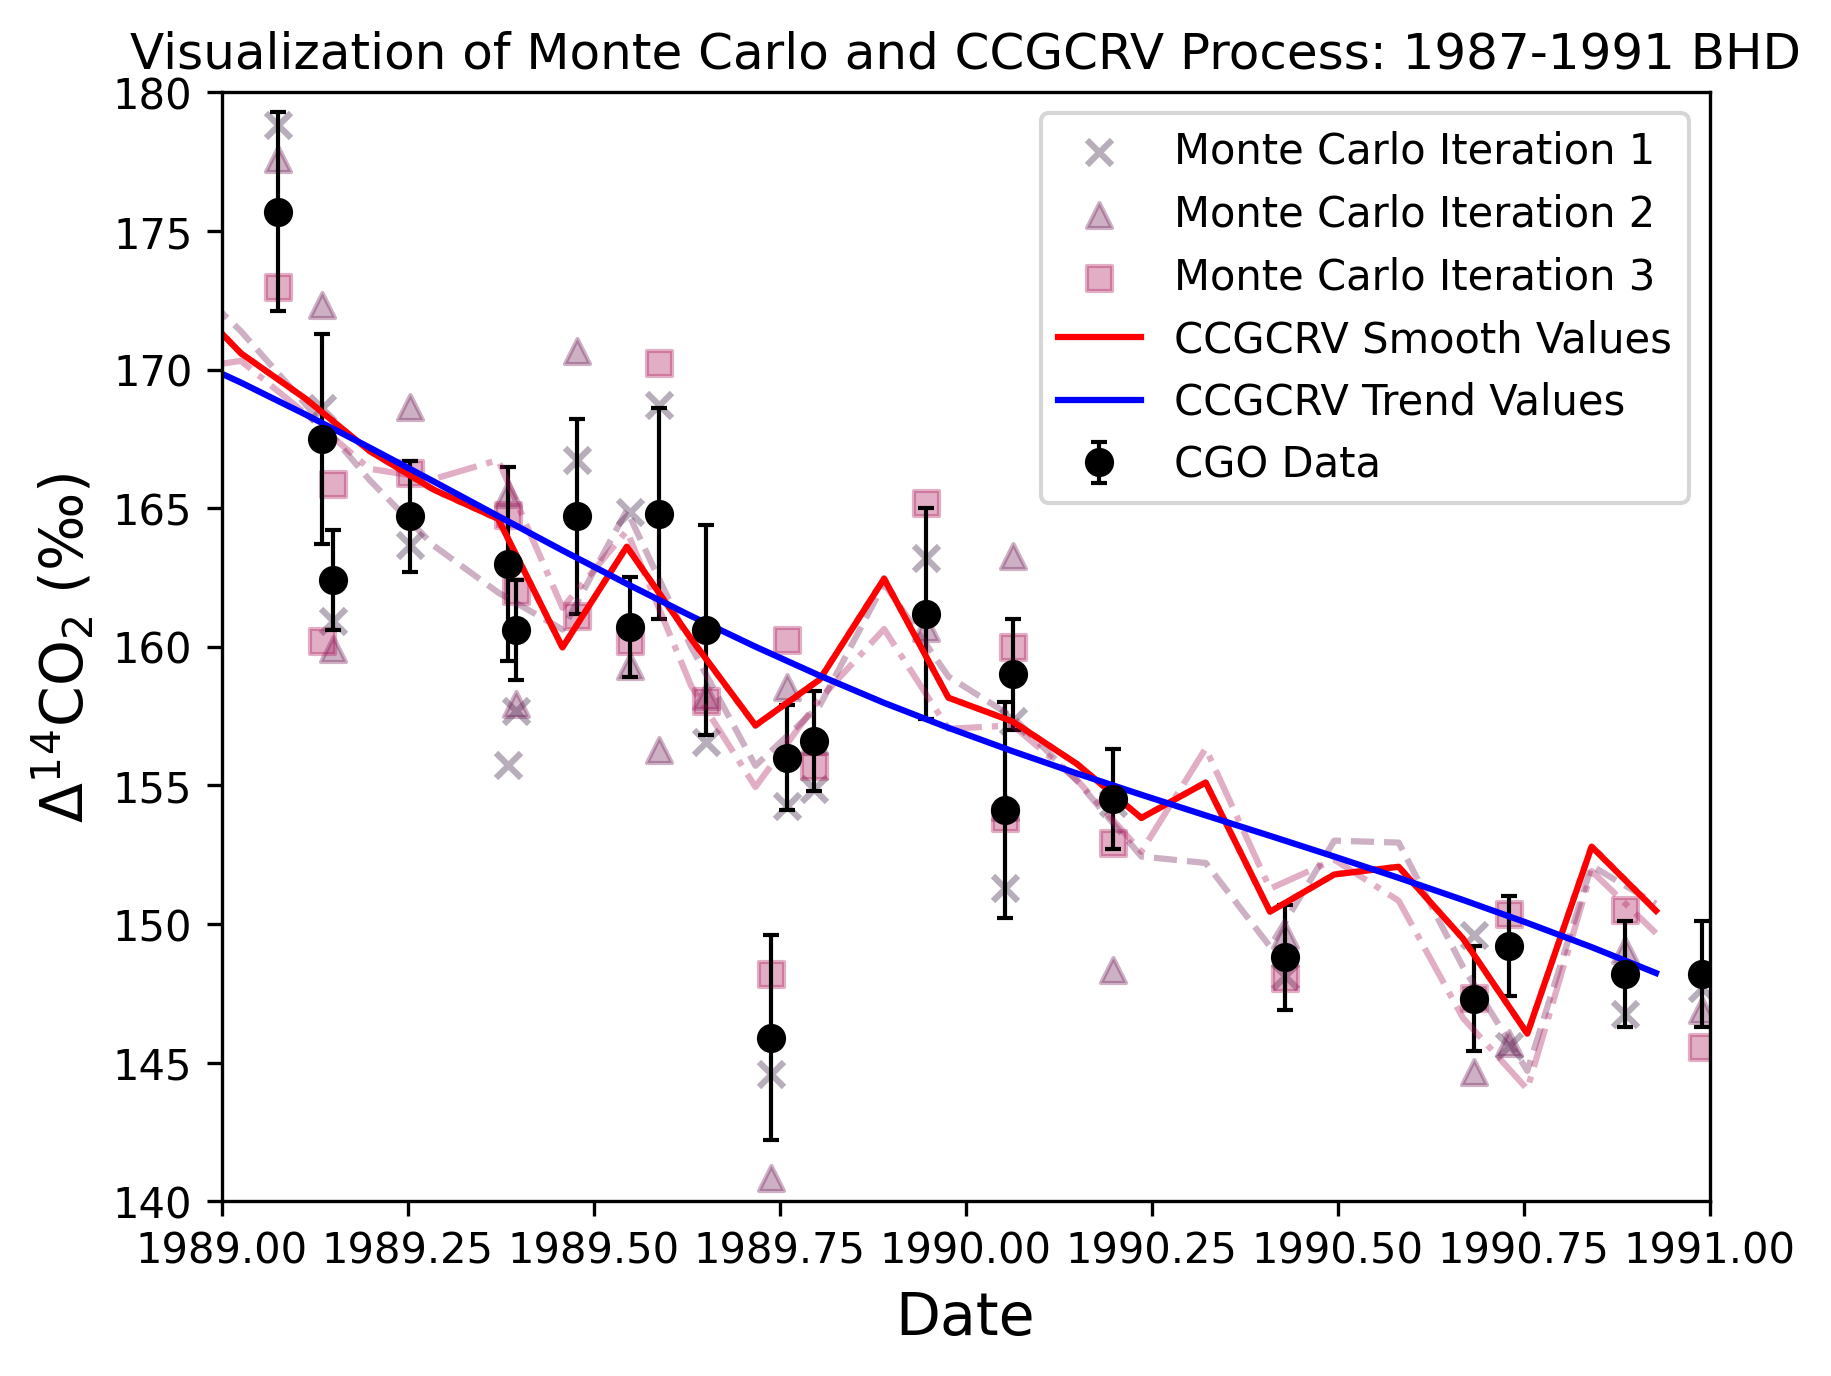
\includegraphics[width=1\textwidth]{/mnt/c/Users/clewis/IdeaProjects/GNS/Interlab_Comparison/output/DEV_FirstDraft_figure2.png}
  \caption{Vizualization of the Monte Carlo simulation to generate an uncertainty estimate about the CCGCRV curve smoothing algoritm. }
  \label{fig:montecarloexplained}
\end{figure}

\subsection{Scripps Institude of Oceaography / Lawrence Livermore National Laboratory}
\subsubsection{Available Data}

RRL and Scripps Institude of Oceaography / Lawrence Livermore National Laboratory (SIO/LLNL) are compared through measurement of the same standard materials: Niwot Ridge 3 and Niwot Ridge 4 (NWT3 and NWT4). NWT3 and NWT4 are air standards from Niwot Ridge, Colorado collected in 2005 and 2006, the latter "spiked" with fossil ${CO_{2}}$. In these particular measurements, standards were graphitized and combusted at SIO and ${\Delta^{14}C}$ measured at LLNL. This intercomparison is sparse in terms of temporal overlap, with RRL measurements ranging from 2013 to 2020; and LLNL measurements encompassing March - April 2009. 
% less than three wheels in reality. 












